
\section{Applications and Domains}
\label{sec:applications}

Implicit and explicit feedback find applications across diverse domains, with feedback types influencing personalization strategies, user experience, and business outcomes. This section provides comprehensive analysis of how different feedback modalities shape recommendation systems in various industries and use cases.

\begin{figure}[ht]
\centering
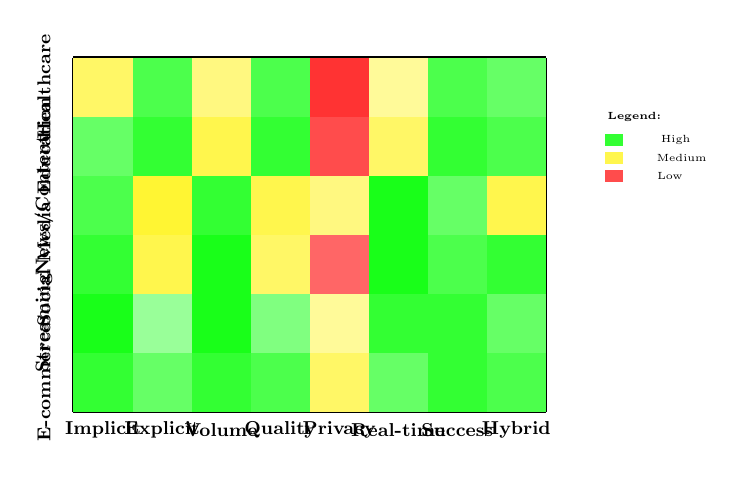
\begin{tikzpicture}[scale=0.75, transform shape]
    % Domain matrix
    \draw[thick] (0,0) grid (8,6);
    
    % Headers
    \node[font=\small\bfseries, rotate=90] at (-0.5,0.5) {E-commerce};
    \node[font=\small\bfseries, rotate=90] at (-0.5,1.5) {Streaming};
    \node[font=\small\bfseries, rotate=90] at (-0.5,2.5) {Social Media};
    \node[font=\small\bfseries, rotate=90] at (-0.5,3.5) {News/Content};
    \node[font=\small\bfseries, rotate=90] at (-0.5,4.5) {Education};
    \node[font=\small\bfseries, rotate=90] at (-0.5,5.5) {Healthcare};
    
    \node[font=\small\bfseries] at (0.5,-0.3) {Implicit};
    \node[font=\small\bfseries] at (1.5,-0.3) {Explicit};
    \node[font=\small\bfseries] at (2.5,-0.3) {Volume};
    \node[font=\small\bfseries] at (3.5,-0.3) {Quality};
    \node[font=\small\bfseries] at (4.5,-0.3) {Privacy};
    \node[font=\small\bfseries] at (5.5,-0.3) {Real-time};
    \node[font=\small\bfseries] at (6.5,-0.3) {Success};
    \node[font=\small\bfseries] at (7.5,-0.3) {Hybrid};
    
    % Content fills
    % E-commerce row
    \fill[green!80] (0,0) rectangle (1,1);
    \fill[green!60] (1,0) rectangle (2,1);
    \fill[green!80] (2,0) rectangle (3,1);
    \fill[green!70] (3,0) rectangle (4,1);
    \fill[yellow!60] (4,0) rectangle (5,1);
    \fill[green!60] (5,0) rectangle (6,1);
    \fill[green!80] (6,0) rectangle (7,1);
    \fill[green!70] (7,0) rectangle (8,1);
    
    % Streaming row
    \fill[green!90] (0,1) rectangle (1,2);
    \fill[green!40] (1,1) rectangle (2,2);
    \fill[green!90] (2,1) rectangle (3,2);
    \fill[green!50] (3,1) rectangle (4,2);
    \fill[yellow!40] (4,1) rectangle (5,2);
    \fill[green!80] (5,1) rectangle (6,2);
    \fill[green!80] (6,1) rectangle (7,2);
    \fill[green!60] (7,1) rectangle (8,2);
    
    % Social Media row
    \fill[green!80] (0,2) rectangle (1,3);
    \fill[yellow!70] (1,2) rectangle (2,3);
    \fill[green!90] (2,2) rectangle (3,3);
    \fill[yellow!60] (3,2) rectangle (4,3);
    \fill[red!60] (4,2) rectangle (5,3);
    \fill[green!90] (5,2) rectangle (6,3);
    \fill[green!70] (6,2) rectangle (7,3);
    \fill[green!80] (7,2) rectangle (8,3);
    
    % News row
    \fill[green!70] (0,3) rectangle (1,4);
    \fill[yellow!80] (1,3) rectangle (2,4);
    \fill[green!80] (2,3) rectangle (3,4);
    \fill[yellow!70] (3,3) rectangle (4,4);
    \fill[yellow!50] (4,3) rectangle (5,4);
    \fill[green!90] (5,3) rectangle (6,4);
    \fill[green!60] (6,3) rectangle (7,4);
    \fill[yellow!70] (7,3) rectangle (8,4);
    
    % Education row
    \fill[green!60] (0,4) rectangle (1,5);
    \fill[green!80] (1,4) rectangle (2,5);
    \fill[yellow!70] (2,4) rectangle (3,5);
    \fill[green!80] (3,4) rectangle (4,5);
    \fill[red!70] (4,4) rectangle (5,5);
    \fill[yellow!60] (5,4) rectangle (6,5);
    \fill[green!80] (6,4) rectangle (7,5);
    \fill[green!70] (7,4) rectangle (8,5);
    
    % Healthcare row
    \fill[yellow!60] (0,5) rectangle (1,6);
    \fill[green!70] (1,5) rectangle (2,6);
    \fill[yellow!50] (2,5) rectangle (3,6);
    \fill[green!70] (3,5) rectangle (4,6);
    \fill[red!80] (4,5) rectangle (5,6);
    \fill[yellow!40] (5,5) rectangle (6,6);
    \fill[green!70] (6,5) rectangle (7,6);
    \fill[green!60] (7,5) rectangle (8,6);
    
    % Legend
    \node[font=\tiny] at (9.5,5) {\textbf{Legend:}};
    \fill[green!80] (9,4.5) rectangle (9.3,4.7);
    \node[font=\tiny] at (10.2,4.6) {High};
    \fill[yellow!70] (9,4.2) rectangle (9.3,4.4);
    \node[font=\tiny] at (10.3,4.3) {Medium};
    \fill[red!70] (9,3.9) rectangle (9.3,4.1);
    \node[font=\tiny] at (10.1,4) {Low};
    
\end{tikzpicture}
\caption{Domain Application Matrix: Feedback Characteristics Across Industries}
\label{fig:domain_matrix}
\end{figure}

Figure~\ref{fig:domain_matrix} provides a comprehensive comparison of feedback characteristics across major application domains, illustrating how different industries leverage implicit and explicit feedback mechanisms with varying degrees of success and privacy considerations.

\subsection{E-commerce and Retail}

\subsubsection{Product Recommendation Systems}

E-commerce platforms leverage complex feedback ecosystems:

\begin{itemize}
    \item \textbf{Implicit Feedback Sources}: Clickstreams, browsing patterns, cart additions, purchase sequences, search queries, and time spent on product pages
    \item \textbf{Explicit Feedback Sources}: Product ratings, detailed reviews, wishlists, and return/refund feedback
    \item \textbf{Hybrid Integration}: Combining browsing intent with review validation for purchase prediction
\end{itemize}

Key challenges include:
\begin{itemize}
    \item \textbf{Abandonment Prediction}: Using implicit signals to identify at-risk shopping carts
    \item \textbf{Cross-Sell Optimization}: Recommending complementary products based on purchase patterns
    \item \textbf{Personalized Pricing}: Dynamic pricing based on user engagement and purchase history
    \item \textbf{Inventory Management}: Demand forecasting using implicit browsing trends
\end{itemize}

\subsubsection{Case Studies}

\textbf{Amazon's Recommendation Engine}:
\begin{itemize}
    \item Processes billions of implicit interactions daily
    \item "Customers who bought this also bought" uses collaborative filtering on purchase data
    \item "Frequently bought together" leverages co-purchase patterns
    \item Explicit reviews influence product ranking and visibility
    \item Hybrid models achieve 35\% of all purchases through recommendations
\end{itemize}

\textbf{Alibaba's Taobao Platform}:
\begin{itemize}
    \item Real-time implicit feedback processing for flash sales
    \item Social commerce integration with explicit friend recommendations
    \item Mobile-optimized implicit feedback (touch gestures, scroll patterns)
    \item Cross-border recommendation challenges with cultural feedback differences
\end{itemize}

\subsubsection{Performance Metrics}

E-commerce success metrics include:
\begin{itemize}
    \item \textbf{Conversion Rate}: Click-to-purchase ratios (typically 2-5\%)
    \item \textbf{Average Order Value}: Revenue impact of recommendations
    \item \textbf{Cart Completion Rate}: Reduction in abandonment through personalized suggestions
    \item \textbf{Return Rate}: Quality of recommendations measured by post-purchase satisfaction
\end{itemize}

\subsection{Content Streaming and Entertainment}

\subsubsection{Video Streaming Platforms}

Netflix, YouTube, and similar platforms rely heavily on implicit feedback:

\begin{itemize}
    \item \textbf{Implicit Signals}: Watch time, completion rates, skip behavior, pause patterns, rewind/fast-forward actions
    \item \textbf{Explicit Signals}: Thumbs up/down, ratings, reviews, playlist creation
    \item \textbf{Contextual Factors}: Time of day, device type, binge-watching patterns
\end{itemize}

Advanced applications include:
\begin{itemize}
    \item \textbf{Content Discovery}: Genre exploration based on viewing patterns
    \item \textbf{Binge Prediction}: Anticipating multi-episode consumption
    \item \textbf{Ad Insertion}: Optimal placement based on engagement patterns
    \item \textbf{Content Creation}: Using feedback to guide production decisions
\end{itemize}

\subsubsection{Music Streaming Services}

Spotify and Apple Music optimize for user engagement:

\begin{itemize}
    \item \textbf{Implicit Feedback}: Play counts, skip rates, playlist additions, repeat listens, share actions
    \item \textbf{Explicit Feedback}: Song ratings, playlist curation, artist follows, concert ticket purchases
    \item \textbf{Temporal Patterns}: Daily routines, mood-based listening, social sharing
\end{itemize}

Key innovations:
\begin{itemize}
    \item \textbf{Discover Weekly}: Algorithmic playlist generation from listening history
    \item \textbf{Blend Playlists}: Social music discovery through shared listening patterns
    \item \textbf{Mood Detection}: Inferring emotional state from music selection patterns
    \item \textbf{Live Performance Prediction}: Concert recommendations based on artist engagement
\end{itemize}

\subsubsection{Case Study: Netflix Recommendation System}

\begin{itemize}
    \item \textbf{Data Scale}: Processes 500+ billion user interactions daily
    \item \textbf{Implicit Dominance}: 95\% of viewing decisions based on implicit feedback
    \item \textbf{Personalized Thumbnails}: A/B testing different artwork based on user preferences
    \item \textbf{Row Personalization}: Dynamic content organization based on viewing history
    \item \textbf{Impact}: Accounts for 80\% of viewing time, prevents churn through engagement
\end{itemize}

\subsection{News and Content Platforms}

\subsubsection{News Recommendation Challenges}

News platforms balance timeliness with quality:

\begin{itemize}
    \item \textbf{Implicit Feedback}: Click-through rates, dwell time, scroll depth, sharing actions
    \item \textbf{Explicit Feedback}: Article ratings, topic preferences, follow actions, report buttons
    \item \textbf{Quality Signals}: Time spent reading, return visits, bookmarking behavior
\end{itemize}

Critical considerations:
\begin{itemize}
    \item \textbf{Filter Bubble Mitigation}: Balancing personalization with diversity
    \item \textbf{Fake News Detection}: Using engagement patterns to identify misinformation
    \item \textbf{Breakthrough Discovery}: Introducing users to new topics and perspectives
    \item \textbf{Real-time Adaptation}: Responding to breaking news and trending topics
\end{itemize}

\subsubsection{Social News Platforms}

Reddit and similar platforms use community feedback:

\begin{itemize}
    \item \textbf{Implicit Signals}: Upvote timing, comment engagement, subreddit subscriptions
    \item \textbf{Explicit Signals}: Direct feedback, moderator actions, community guidelines
    \item \textbf{Social Dynamics}: Influence propagation through social networks
\end{itemize}

\subsection{Social Media and Networking}

\subsubsection{Content Ranking Algorithms}

Facebook, Twitter, and Instagram optimize for engagement:

\begin{itemize}
    \item \textbf{Implicit Feedback}: Likes, shares, comments, view duration, profile visits
    \item \textbf{Explicit Feedback}: Follow/unfollow actions, content reports, privacy settings
    \item \textbf{Network Effects}: Social graph analysis and influence propagation
\end{itemize}

Key applications:
\begin{itemize}
    \item \textbf{Feed Personalization}: Algorithmic content ranking for individual users
    \item \textbf{Ad Targeting}: Precise audience segmentation based on behavioral patterns
    \item \textbf{Community Detection}: Identifying interest groups and social clusters
    \item \textbf{Influence Maximization}: Optimizing content spread through social networks
\end{itemize}

\subsubsection{Case Study: Twitter's Algorithm}

\begin{itemize}
    \item \textbf{Multi-Objective Optimization}: Balancing engagement, relevance, and recency
    \item \textbf{Implicit Signals}: Retweet patterns, quote tweet behavior, thread engagement
    \item \textbf{Real-time Processing}: Adapting to trending topics and breaking news
    \item \textbf{Conversation Health}: Promoting constructive dialogue through feedback analysis
\end{itemize}

\subsection{Emerging Domains and Applications}

\subsubsection{Educational Platforms}

Learning management systems use feedback for personalization:

\begin{itemize}
    \item \textbf{Implicit Feedback}: Time spent on materials, quiz attempt patterns, navigation sequences
    \item \textbf{Explicit Feedback}: Course ratings, assignment feedback, learning goal declarations
    \item \textbf{Adaptive Learning}: Personalizing content difficulty and pacing based on engagement
\end{itemize}

\subsubsection{Health and Fitness Applications}

Wellness apps optimize for behavior change:

\begin{itemize}
    \item \textbf{Implicit Feedback}: Workout completion, step counts, sleep patterns, app usage frequency
    \item \textbf{Explicit Feedback}: Goal setting, satisfaction surveys, pain level reporting
    \item \textbf{Motivation Systems}: Using engagement patterns to provide timely encouragement
\end{itemize}

\subsubsection{Professional Networking}

LinkedIn and similar platforms focus on career development:

\begin{itemize}
    \item \textbf{Implicit Feedback}: Profile view patterns, connection requests, content engagement
    \item \textbf{Explicit Feedback}: Endorsements, recommendations, skill assessments
    \item \textbf{Career Path Prediction}: Using interaction patterns to suggest professional development
\end{itemize}

\subsubsection{Gaming and Interactive Entertainment}

Game platforms personalize player experiences:

\begin{itemize}
    \item \textbf{Implicit Feedback}: Play time, level completion, in-game purchases, social interactions
    \item \textbf{Explicit Feedback}: Game ratings, review comments, friend recommendations
    \item \textbf{Dynamic Difficulty}: Adjusting challenge levels based on player skill patterns
\end{itemize}

\subsection{Domain-Specific Feedback Characteristics}

\subsubsection{Feedback Abundance and Quality}

Different domains exhibit varying feedback landscapes:

\begin{table}[h]
\centering
\caption{Feedback Characteristics Across Domains}
\label{tab:domain_feedback}
\begin{tabular}{@{}lcccc@{}}
\toprule
Domain & Implicit Volume & Explicit Quality & Real-time Needs & Privacy Sensitivity \\
\midrule
E-commerce & Very High & High & Medium & Medium \\
Video Streaming & Extremely High & Medium & High & Low \\
Music Streaming & High & Medium & High & Low \\
News & High & Low & Very High & Medium \\
Social Media & Very High & Low & Very High & High \\
Education & Medium & High & Low & High \\
Health/Fitness & High & Medium & Medium & Very High \\
Professional & Medium & High & Low & High \\
Gaming & High & Medium & High & Medium \\
\bottomrule
\end{tabular}
\end{table}

\subsubsection{Cross-Domain Feedback Transfer}

Understanding feedback patterns across domains enables transfer learning:

\begin{itemize}
    \item \textbf{Music to Video}: Audio preferences predicting visual content interests
    \item \textbf{Shopping to Entertainment}: Purchase patterns informing content recommendations
    \item \textbf{Social to Professional}: Network behavior patterns in career contexts
    \item \textbf{Educational to Gaming}: Learning patterns informing game personalization
\end{itemize}

\subsection{Industry Best Practices and Implementation}

\subsubsection{Data Pipeline Architecture}

Successful implementations require robust infrastructure:

\begin{itemize}
    \item \textbf{Real-time Processing}: Streaming analytics for immediate feedback incorporation
    \item \textbf{Scalable Storage}: Distributed databases handling massive feedback volumes
    \item \textbf{Privacy Compliance}: GDPR/CCPA-compliant data handling and user consent management
    \item \textbf{A/B Testing Frameworks}: Continuous experimentation and performance monitoring
\end{itemize}

\subsubsection{Model Deployment and Monitoring}

Production systems require careful management:

\begin{itemize}
    \item \textbf{Online Learning}: Continuous model updates with new feedback
    \item \textbf{Performance Monitoring}: Real-time tracking of recommendation quality metrics
    \item \textbf{Fallback Strategies}: Graceful degradation when feedback signals are weak
    \item \textbf{Bias Detection}: Ongoing monitoring for unfair or discriminatory patterns
\end{itemize}

\subsubsection{User Experience Optimization}

Feedback integration affects user satisfaction:

\begin{itemize}
    \item \textbf{Seamless Integration}: Implicit feedback collection without disrupting user flow
    \item \textbf{Transparency}: Clear communication about how feedback influences recommendations
    \item \textbf{Control Mechanisms}: User options to adjust feedback sensitivity and preferences
    \item \textbf{Privacy Controls}: Granular permissions for different feedback types
\end{itemize}

\subsection{Impact on Business Outcomes}

\subsubsection{Quantitative Benefits}

Successful feedback integration drives measurable improvements:

\begin{itemize}
    \item \textbf{Revenue Impact}: 15-35\% increase in conversion rates through personalized recommendations
    \item \textbf{User Engagement}: 20-50\% improvement in session duration and return visits
    \item \textbf{Customer Satisfaction}: Higher NPS scores through relevant personalization
    \item \textbf{Operational Efficiency}: Reduced support costs through proactive recommendations
\end{itemize}

\subsubsection{Qualitative Benefits}

Beyond metrics, feedback systems provide strategic advantages:

\begin{itemize}
    \item \textbf{Competitive Differentiation}: Superior personalization as a market advantage
    \item \textbf{Customer Loyalty}: Building long-term relationships through understanding
    \item \textbf{Innovation Opportunities}: Data-driven insights for product development
    \item \textbf{Risk Mitigation}: Early detection of user dissatisfaction and churn signals
\end{itemize}

\subsection{Future Domain Evolution}

Emerging trends will reshape feedback utilization:

\begin{itemize}
    \item \textbf{Metaverse Integration}: Spatial and embodied feedback in virtual environments
    \item \textbf{IoT Ecosystem}: Connected device feedback for holistic user understanding
    \item \textbf{Brain-Computer Interfaces}: Direct neural feedback for ultimate personalization
    \item \textbf{Quantum Computing}: Massive-scale feedback processing for unprecedented accuracy
\end{itemize}

This comprehensive analysis demonstrates how feedback types fundamentally shape recommendation system design and outcomes across diverse application domains, with each domain requiring tailored approaches to maximize effectiveness and user satisfaction.
